\documentclass[conference]{IEEEtran}
\IEEEoverridecommandlockouts
% The preceding line is only needed to identify funding in the first footnote. If that is unneeded, please comment it out.
\usepackage{cite}
%\usepackage{hyperref}
\usepackage{amsmath,amssymb,amsfonts}
\usepackage{algorithmic}
\usepackage{graphicx} \usepackage{textcomp}
\usepackage{xcolor, soul}
\sethlcolor{gray}
\usepackage{url}
\usepackage{cleveref}
\def\BibTeX{{\rm B\kern-.05em{\sc i\kern-.025em b}\kern-.08em
    T\kern-.1667em\lower.7ex\hbox{E}\kern-.125emX}}
\begin{document}

\title{Project 7: Studying  ISIS Twitter influence with social network analysis from the pro-ISIS fanboy tweet data}
%{\footnotesize \textsuperscript{*}Note: Sub-titles are not captured in Xplore and
%should not be used}
%}




\author{\IEEEauthorblockN{1\textsuperscript{st} Niklas Saari}
    \IEEEauthorblockA{\textit{dept. Computer Science and Engineering} \\
        \textit{University of Oulu}\\
        Oulu, Finland \\
        niklas.saari@student.oulu.fi}
}

\maketitle

\begin{abstract}
    This document describes project work for the course Social Network Analysis in Spring 2021.
    Radical and extreme groups have taken social networks as part of their toolchain to spread propaganda messages,
    get attention, look support for their actions and recruit more members.
    One of the most brutal of these groups, ISIS, which is also designated as terrorist organization, has been forerunner on using these social platforms successfully.
    To possibly prevent future terror events, it would be important to study these social networks on how they are used by these radical groups.
    ISIS Twitter dataset of around 17~000 tweets was selected as dataset to identify important characters from the network, to construct communities and to see how the most influencers behave, who they are, and how they connect to other people.
    Further communities were constructed to see how networks behave internally.

\end{abstract}

\begin{IEEEkeywords}
    Twitter, Social Network Analysis, Terrorism, Networks, ISIS
\end{IEEEkeywords}

\section{Group information}\label{sec:group-description}

This project has been done alone.
The original project from the given project list was 7 with the title of "Analysis of ISIS Twitter dataset".

\section{Introduction}\label{sec:introduction}

Social networks have become part of the most people's everyday life.
These networks, such as Facebook, Twitter or Reddit are base for many kinds of groups and people for communicating with each other.
They are being used widely for expressing opinions or advertising services and for many other kinds of things.
This has naturally risen special interest in radical and terrorism organisations because of the provided possibility for
influencing different kind of people with a large scale.
While the brutality of terrorism has become even more severe over recent time based on the data gathered by Global
Terrorism Database and seen in Appendixes in the figure \ref{fig:appendix_terrorism_deaths}, this raises specific interest
in terms of identifying and preventing possible future incidents.

Terrorism is identified to be especially brutal from Islamic State of Iraq and Levant (ISIL), which is also known ISIS
or Daesh.\cite{enwiki:1024074085}
Their usage of the social media is also known to be "probably more sophisticated than [that of] most US companies",\cite{isis-selling-terror}
and has been one of their main campaigning tactics in Syria and Iraq.
Twitter has been their primal social network\cite{isis-how-twitter} so far.
It is known that ISIS has been previously organising for example specific hashtag campaigns to get their topics
trending and gain more visibility\cite{isis-how-twitter}.

Because the social networks have begun to be in key role to motivate support for their actions, raise funds and even for recruiting
foreign fighters with huge success\cite{isis-foreign-fighter} allowing organisation to reach worldwide recognition and impact,
it is important to study how these networks are formed and what we could learn from them and how we could act based on this information.

Social Network Analysis (SNA) is a process for studying social life by social structures which is constructed by relations and patterns formed by these relations.
This is usually done with networks and applying the graph theory.\cite{marin2011social, doi:10.1177/016555150202800601}

In this article we will focus particularly on the Twitter platform and for the Social Network Analysis of how ISIS  has been using this specific
platform to spread their propaganda and organizing recruitment.
Twitter data of over 17~000 tweets of pro-ISIS fanboys has been used as dataset for this study.

We will try to identify major characters from the provided data, for example which characters have the most influence and
what kind of networks they are constructing.
This is evaluated based on different values specific for Twitter platform, such as usage of mentions, retweets or hashtags; how are different Twitter users using them.

We further try to estimate the sentiment of the tweets in terms of negative, neutral and positive and estimate the most
frequent hashtags and their possible context and characteristics.
Sentiments are finally plotted with ternary plots by different characteristics.
Different kind of other graphs will be constructed to develop our understanding of underlying network.
Social network is constructed by using hashtags, and their relations to other tweets based on their appearances.

This document is structured as following: in the section~\ref{sec:problem-description} the main problem has been described.
In the section~\ref{sec:dataset-description} the exact details of the used dataset has been described.
In the section~\ref{sec:general-methodology} general methodology has been described and further continued in the section~\ref{sec:detailed-methodology}
in more precise matter.
The results are presented in the section~\ref{sec:results-and-discussion} and paper has been finally concluded in the section~\ref{sec:conclusion-and-perspectives}.

\section{Problem Description}\label{sec:problem-description}

The main problem is to study and tell how we can find specific communities from underlying dataset and identify interesting
numerical values from the constructed network.
Can we detect specific patterns or behaviours related to specific Twitter users, is there connection between them and how powerful their influence actually is?
We further try to find a way to tell about what kind of messages they are distributing in overall.
Dataset was not collected by itself, instead it was given in the project assignment.

\section{Dataset description}\label{sec:dataset-description}

Twitter dataset of tweets collected from pro-ISIS fanboys of all over the world has been used as a base for this study.
This dataset was provided with the project assigment.
Based on the same project assigment, the origin of the dataset is unknown, as it is stated to be published in dark web website.
However, after doing some research, it seems that this dataset is probably collected by Fifth Tribe digital agency, and published originally on the \textit{Kaggle.}\cite{dataKaggleOrigin}
Data is under Creative Commons 0 (CC0) license and can be used without restrictions to the fullest extent allowed by law.
Data was created originally with the intention of "to develop effective counter-messaging measures against violent extremists at home and abroad."\cite{dataKaggleOrigin}

Tweets are located during the period of 1st of June 2015 and 13rd of May 2016, which contains the November 2015 Paris attack as interesting
point of event regarding the context of this study.
Tweets are had been written with multiple languages, but in general they are in English.
Their content is varying a lot; they could be text with varying context, external links to other places, images and videos or rewteets.

Dataset contains total of 17410 different tweets by 112 different users, and was originally given in the newer Excel format (\textbf{.xlsx}).
Following data columns can be found from the raw data:

\begin{itemize}
    \item name
    \item username
    \item location
    \item number of followers
    \item number of statuses
    \item time (month/day/year 24-hour clock)
    \item tweet (multilingual)
\end{itemize}

Location is user supplied data and can be therefore anything.

\subsection{Pre-processing of the data}\label{subsec:pre-processing-of-the-data}

As the initial dataset was given in Microsoft Excel Open XML (.xlsx) format, it required some conversion to be more suitable for processing with
programmatically with selected programming language (Python in this case) and in general for easier handling and compatibility.
Dataset was converted to basic \textbf{.csv} file format by using Python \textbf{pandas}\cite{mckinney2010data} library with \textbf{openpyxl}\cite{openpyxl} engine.
Successful conversion was verified later by checking that there were no null data shells for columns which are considered as "important" and the amount of rows matches with original and converted data.
"Important" means in this context that every tweet should have at least username and tweet content to be meaningful.

The data has been on some cases further pre-processed as following to extract some specific information and features.
This information is stored programmatically on the run-time-memory by creating specific Python class object to represent single line from the dataset data, which also contains extracted additional data.
Extracting methods have been discussed in more detail on the section~\ref{sec:detailed-methodology}.

\subsubsection{Mentions}

Mentions of different users have been extracted from the every tweet based on the '@' symbol in tweet data.
Twitter usernames are case-insensitive and therefore as and additional step, they are stored in lowercase to improve accuracy of the data and also to reflect real world behaviour when linking to other tweets.
This is implemented by using specific regex patterns.

\subsubsection{Retweets}

Retweets are identified from the data based on 'RT' as first word in the tweet.

\subsubsection{Hashtags}

Hashtags have been extracted from the every tweet based on the '\#' symbol in tweet data.
Twitter hashtags are case-insensitive and therefore as and additional step, they are stored in lowercase to improve accuracy of the data and also to reflect real world behaviour when linking to other tweets.
This is implemented by using specific regex patterns.


\subsubsection{Sentiment analysis}

Sentiment analysis is applied for every tweet in the dataset to describe the potential category in terms of \textit{negative, neutral and positive.}
Python package named as VADER Sentiment, which was originally presented in the article "VADER: A Parsimonious Rule-Based Model for Sentiment Analysis of Social Media Text"\cite{Hutto_Gilbert_2014} has been used as tool for scoring the data for these categories.
This is discussed in more details on the section~\ref{sec:detailed-methodology}.

\subsection{Data verification after pre-processing methods}


As there were many methods implemented for extracting information from the dataset, some testcases were applied
and random data was selected to be sure, that extraction is working as expected.
This was also applied for data conversion.
Testing was implemented by using Python package \textbf{pytest}\cite{pytestx.y}, and based on the limited test cases data is extracted as intended.

\section{General methodology}\label{sec:general-methodology}

In general, the methodology on study is based on processing the Twitter dataset with Python programming language and selected existing libraries.
Dataset was pre-processed at first to convert it to suitable format and further some methods are applied to extract
features from the tweets, such as hashtags or mentions, as mentioned in the section~\ref{sec:dataset-description}.


NetworkX\cite{SciPyProceedings_11} is the main package used in the work.
It is mainly used to "study structure" or other properties of potentially complex networks.
In this scenario it is used to construct a network model based on appearing hashtags in Twitter tweets.
Some properties have been measured from the constructed network to make conclusions based on that.

Matplotlib\cite{4160265} is the main library used for drawing the visible graphs in this document.

Vader Sentiment\cite{Hutto_Gilbert_2014} tool has been used to identify sentiment of the every tweet on some occurrences.

\section{Detailed methodology}\label{sec:detailed-methodology}

This section is going through exact details of the process how data was handled and how results were finally obtained.
Actual results are described later on the section~\ref{sec:results-and-discussion}.


\subsection{Initial steps}

To get started with the analysis our Twitter data, we are required to shape data suitable for our use case.
This was briefly described in the section~\ref{sec:dataset-description} on "preprocessing" subsection.
Data was converted into \textbf{.csv} format and loaded into program memory.

Initially, specific Python class was designed to allow ease access for tweet data and feature extraction.
UML diagram can be seen in the figure~\ref{fig:tweetdata_design}.
This class has build-in methods for extracting specific features from the tweet data and it converts values to suitable data types e.g. time into build-in Python time object.
Methods include extracting hashtags, mentions and identification is the tweet retweet, and evaluation of possible sentiment value of it.

\begin{figure}
    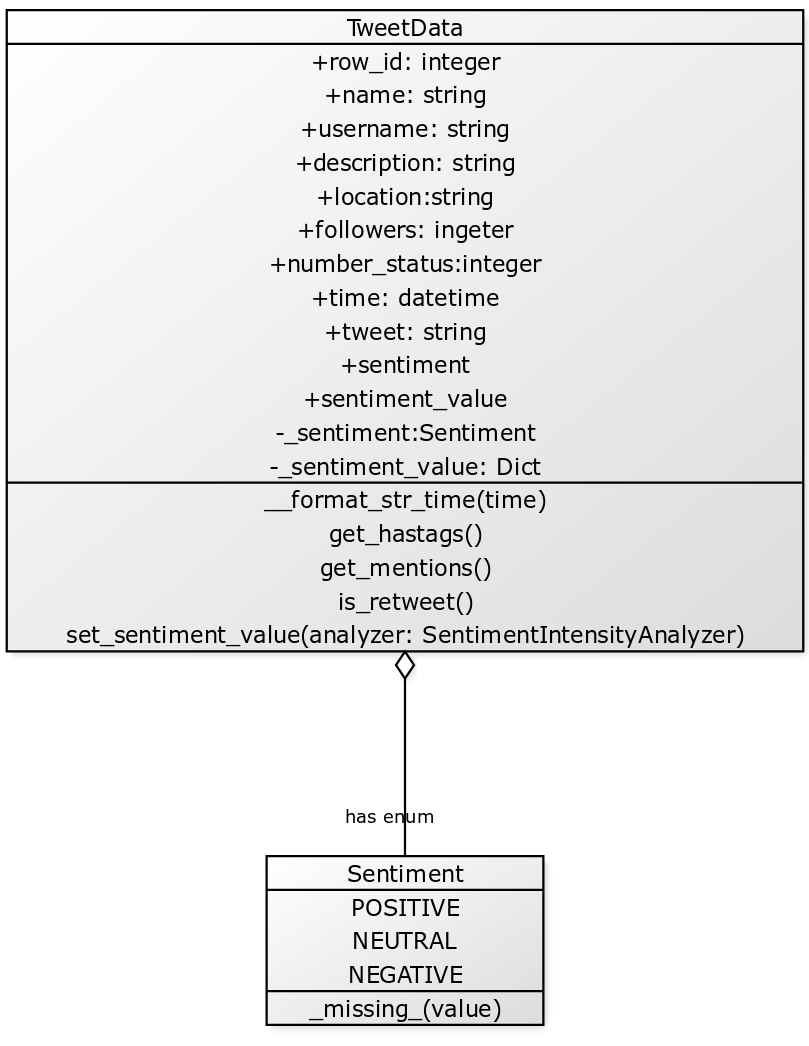
\includegraphics[scale=0.3]{figures/uml_tweetdata}
    \caption{Designed class for storing and handling the Tweet data}
    \label{fig:tweetdata_design}
\end{figure}

Sentiment analysis is used here to make mass analysis for all tweets to categorize every tweet for one of the NEGATIVE, NEUTRAL and POSITIVE semantic orientations.
This is useful stat to generalize what kind message(s) individuals are tweeting.

Individual Twitter users will be sorted and handled separately by using different metrics: by use of the retweets, mentions and use of hashtags.
Also, sentiments among all the tweets will be evaluated.
VADER (Valence  Aware  Dictionary  for  sEntiment  Reasoning) tool\cite{Hutto_Gilbert_2014} has been used for making the sentiment calculation.
It was released in 2014 and has acquired fame from its efficiency and accuracy.
By default, tool is producing four different values for provided input as results.
Three of the values (pos, neu and neg) are pointing the portion of the three orientations, from range to 0 into 1, totalling to sum of 1.
One is describing overall result (compound), which "is computed by summing the valence scores of each word in the lexicon, adjusted according to the rules, and then normalized to be between -1 (most extreme negative) and +1 (most extreme positive)."

Therefore, sentiment orientation is finally defined by compound value as following:

\begin{center}
\begin{tabular}{ |c|c|c| }
 \hline
 score $\geq$ 0.05 & Positive sentiment \\
 \hline
 score $>$ -0.05 & Neutral sentiment \\
 \hline
 score $\leq$ -0.05 & Negative sentiment \\
 \hline
\end{tabular}
\end{center}

This classification is implemented on the Sentiment enum in the figure~\ref{fig:tweetdata_design}.
It is giving one of the three sentiment description for every tweet based on calculated compound value, automatically.

Ternary plots are used to describe the results, as they often can give clear visual evidence which variable from the three is  thecontrolling one.
During the assessment of class creation, it was observed that instancing SentimentIntensityAnalyzer from Vader tool is resource consuming, hence
analyzer is instanced only once outside TweetData class and passed into object afterwards to significantly increase performance.


After we have loaded the \textbf{.csv} file, it is parsed in a such a way that from each row in the data, new instance
of TweetData object has been created and list form them is formed.
Further, this list is processed in such a way, that every Twitter user is separated to be part of the new
$<$username$>$:USER\_META dictionary object, which has following attributes; amount\_tweets, amount\_retweets, amount\_mentions, amount\_hashtags and all the tweets this user has tweeted.
This gives us access by username for metadata and user-specific tweets.

Some specific functions have been additionally created that previously created dictionary can be easily sorted, based on it's key-value attributes and finally plotted with suitable graphs.

\subsection{Visualising interesting information}

At this point we already have access for many interesting information.
We can plot and sort users based on their amount of tweets, amount of retweets, amount of mentions and by the amount of hashtag usages.
Matplotlib Python package has been used for this.

We are also interested to know, whether power law is applying here, in the context of tweets by single user.
Power law is known to be functional relationship between two quantities, where probability distributions are often "heavy-tailed".
Pareto principle (80-20) is commonly used as rule to see if data fits under power law\cite{enwiki:1023956740}.

Probability distribution of power law can be seen as

 \begin{equation}
 p(x) \propto x^{-\alpha}\label{eq:equation1}
 \end{equation}

where $\alpha$ is a constant known usually as scaling parameter and \textit{x} as quantity.
Quantity \textit{x} obeys the power law if it is drawn from this distribution.\cite{doi:10.1137/070710111}

Following



Power law

\subsection{Degree Centrality}

Degree centrality is the sum of in-degree and out-degree. 
It is representing the amount of edges entering and leaving the nodes respectively. 
The most important nodes have the most direct connections with others under degree centrality.
The value can be computed as,

\begin{equation*}\label{eq:degree-centrality}
    C_{D}(v_{i})={\sum}_{j}A_{ij} \tag{1} 
\end{equation*}

\subsection{Betweeness Centrality}

Betweeness centrality is another way to measure importance of nodes.
It is describing the amount of the shortest path passing the node.
Important nodes have high betweeness centrality, information is flowing through them, and they are connecting multiple nodes into the network.

\begin{equation*}
    C_{B}(v_{i})={\sum}_{v_{s}\neq v_{i}\neq v_{t}\in V,s < \text{t}}\frac{\sigma_{st}(v_{i})}{\sigma_{st}} \tag{2}
\end{equation*}

\section{Results and Discussion}\label{sec:results-and-discussion}

Initial dataset contained more than 17~000 tweets and 114 different users.
Distribution of the tweets per single user can be seen on the figure~\ref{fig:amount-tweets-user}.

This data distribution seems to be quite "heavy-tailed" which is typical in power law theory, but for further clarification, it was fitted into probability distribution function.


\begin{figure}
    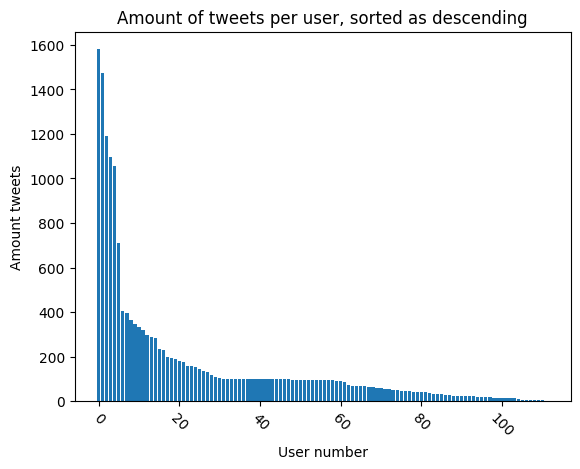
\includegraphics[scale=0.6]{figures/amount_tweets_per_user}
     \caption{Amount of tweets per user}
    \label{fig:amount-tweets-user}
\end{figure}

\section{Conclusion and Perspectives}\label{sec:conclusion-and-perspectives}

%\subsection{Units}
%\begin{itemize}
%    \item Use either SI (MKS) or CGS as primary units. (SI units are encouraged.) English units may be used as secondary units (in parentheses). An exception would be the use of English units as identifiers in trade, such as ``3.5-inch disk drive''.
%    \item Avoid combining SI and CGS units, such as current in amperes and magnetic field in oersteds. This often leads to confusion because equations do not balance dimensionally. If you must use mixed units, clearly state the units for each quantity that you use in an equation.
%    \item Do not mix complete spellings and abbreviations of units: ``Wb/m\textsuperscript{2}'' or ``webers per square meter'', not ``webers/m\textsuperscript{2}''. Spell out units when they appear in text: ``. . . a few henries'', not ``. . . a few H''.
%    \item Use a zero before decimal points: ``0.25'', not ``.25''. Use ``cm\textsuperscript{3}'', not ``cc''.)
%\end{itemize}

%Number equations consecutively. To make your
%equations more compact, you may use the solidus (~/~), the exp function, or
%appropriate exponents. Italicize Roman symbols for quantities and variables,
%but not Greek symbols. Use a long dash rather than a hyphen for a minus
%sign. Punctuate equations with commas or periods when they are part of a
%sentence, as in:
%\begin{equation}
%    a+b=\gamma\label{eq}
%\end{equation}
%
%Be sure that the
%symbols in your equation have been defined before or immediately following
%the equation. Use ``\eqref{eq}'', not ``Eq.~\eqref{eq}'' or ``equation \eqref{eq}'', except at
%the beginning of a sentence: ``Equation \eqref{eq} is . . .''


%Please use ``soft'' (e.g., \verb|\eqref{Eq}|) cross references instead
%of ``hard'' references (e.g., \verb|(1)|). That will make it possible
%to combine sections, add equations, or change the order of figures or
%citations without having to go through the file line by line.
%
%Please don't use the \verb|{eqnarray}| equation environment. Use
%\verb|{align}| or \verb|{IEEEeqnarray}| instead. The \verb|{eqnarray}|
%environment leaves unsightly spaces around relation symbols.
%
%Please note that the \verb|{subequations}| environment in {\LaTeX}
%will increment the main equation counter even when there are no
%equation numbers displayed. If you forget that, you might write an
%article in which the equation numbers skip from (17) to (20), causing
%the copy editors to wonder if you've discovered a new method of
%counting.
%
%    {\BibTeX} does not work by magic. It doesn't get the bibliographic
%data from thin air but from .bib files. If you use {\BibTeX} to produce a
%bibliography you must send the .bib files.
%
%    {\LaTeX} can't read your mind. If you assign the same label to a
%subsubsection and a table, you might find that Table I has been cross
%referenced as Table IV-B3.
%
%{\LaTeX} does not have precognitive abilities. If you put a
%\verb|\label| command before the command that updates the counter it's
%supposed to be using, the label will pick up the last counter to be
%cross referenced instead. In particular, a \verb|\label| command
%should not go before the caption of a figure or a table.
%
%Do not use \verb|\nonumber| inside the \verb|{array}| environment. It
%will not stop equation numbers inside \verb|{array}| (there won't be
%any anyway) and it might stop a wanted equation number in the
%surrounding equation.
%
%\subsection{Some Common Mistakes}\label{SCM}
%\begin{itemize}
%    \item The word ``data'' is plural, not singular.
%    \item The subscript for the permeability of vacuum $\mu_{0}$, and other common scientific constants, is zero with subscript formatting, not a lowercase letter ``o''.
%    \item In American English, commas, semicolons, periods, question and exclamation marks are located within quotation marks only when a complete thought or name is cited, such as a title or full quotation. When quotation marks are used, instead of a bold or italic typeface, to highlight a word or phrase, punctuation should appear outside of the quotation marks. A parenthetical phrase or statement at the end of a sentence is punctuated outside of the closing parenthesis (like this). (A parenthetical sentence is punctuated within the parentheses.)
%    \item A graph within a graph is an ``inset'', not an ``insert''. The word alternatively is preferred to the word ``alternately'' (unless you really mean something that alternates).
%    \item Do not use the word ``essentially'' to mean ``approximately'' or ``effectively''.
%    \item In your paper title, if the words ``that uses'' can accurately replace the word ``using'', capitalize the ``u''; if not, keep using lower-cased.
%    \item Be aware of the different meanings of the homophones ``affect'' and ``effect'', ``complement'' and ``compliment'', ``discreet'' and ``discrete'', ``principal'' and ``principle''.
%    \item Do not confuse ``imply'' and ``infer''.
%    \item The prefix ``non'' is not a word; it should be joined to the word it modifies, usually without a hyphen.
%    \item There is no period after the ``et'' in the Latin abbreviation ``et al.''.
%    \item The abbreviation ``i.e.'' means ``that is'', and the abbreviation ``e.g.'' means ``for example''.
%\end{itemize}
%An excellent style manual for science writers is \cite{b7}.

\subsection{Authors and Affiliations}
%\textbf{The class file is designed for, but not limited to, six authors.} A
%minimum of one author is required for all conference articles. Author names
%should be listed starting from left to right and then moving down to the
%next line. This is the author sequence that will be used in future citations
%and by indexing services. Names should not be listed in columns nor group by
%affiliation. Please keep your affiliations as succinct as possible (for
%example, do not differentiate among departments of the same organization).

\subsection{Identify the Headings}
%Headings, or heads, are organizational devices that guide the reader through
%your paper. There are two types: component heads and text heads.
%
%Component heads identify the different components of your paper and are not
%topically subordinate to each other. Examples include Acknowledgments and
%References and, for these, the correct style to use is ``Heading 5''. Use
%``figure caption'' for your Figure captions, and ``table head'' for your
%table title. Run-in heads, such as ``Abstract'', will require you to apply a
%style (in this case, italic) in addition to the style provided by the drop
%down menu to differentiate the head from the text.
%
%Text heads organize the topics on a relational, hierarchical basis. For
%example, the paper title is the primary text head because all subsequent
%material relates and elaborates on this one topic. If there are two or more
%sub-topics, the next level head (uppercase Roman numerals) should be used
%and, conversely, if there are not at least two sub-topics, then no subheads
%should be introduced.

\subsection{Figures and Tables}
%\paragraph{Positioning Figures and Tables} Place figures and tables at the top and
%bottom of columns. Avoid placing them in the middle of columns. Large
%figures and tables may span across both columns. Figure captions should be
%below the figures; table heads should appear above the tables. Insert
%figures and tables after they are cited in the text. Use the abbreviation
%``Fig.~\ref{fig}'', even at the beginning of a sentence.
%
%\begin{table}[htbp]
%    \caption{Table Type Styles}
%    \begin{center}
%        \begin{tabular}{|c|c|c|c|}
%            \hline
%            \textbf{Table} & \multicolumn{3}{|c|}{\textbf{Table Column Head}}                                                         \\
%            \cline{2-4}
%            \textbf{Head}  & \textbf{\textit{Table column subhead}}           & \textbf{\textit{Subhead}} & \textbf{\textit{Subhead}} \\
%            \hline
%            copy           & More table copy$^{\mathrm{a}}$                   &                           &                           \\
%            \hline
%            \multicolumn{4}{l}{$^{\mathrm{a}}$Sample of a Table footnote.}
%        \end{tabular}
%        \label{tab1}
%    \end{center}
%\end{table}

%\begin{figure}[htbp]
%    \centerline{
\includegraphics{fig1.png}}
%    \caption{Example of a figure caption.}
%    \label{fig}
%\end{figure}

%Figure Labels: Use 8 point Times New Roman for Figure labels. Use words
%rather than symbols or abbreviations when writing Figure axis labels to
%avoid confusing the reader. As an example, write the quantity
%``Magnetization'', or ``Magnetization, M'', not just ``M''. If including
%units in the label, present them within parentheses. Do not label axes only
%with units. In the example, write ``Magnetization (A/m)'' or ``Magnetization
%\{A[m(1)]\}'', not just ``A/m''. Do not label axes with a ratio of
%quantities and units. For example, write ``Temperature (K)'', not
%``Temperature/K''.

\section*{Acknowledgment}

%The preferred spelling of the word ``acknowledgment'' in America is without
%an ``e'' after the ``g''. Avoid the stilted expression ``one of us (R. B.
%G.) thanks $\ldots$''. Instead, try ``R. B. G. thanks$\ldots$''. Put sponsor
%acknowledgments in the unnumbered footnote on the first page.


%Please number citations consecutively within brackets \cite{b1}. The
%sentence punctuation follows the bracket \cite{b2}. Refer simply to the reference
%number, as in \cite{b3}---do not use ``Ref. \cite{b3}'' or ``reference \cite{b3}'' except at
%the beginning of a sentence: ``Reference \cite{b3} was the first $\ldots$''
%
%Number footnotes separately in superscripts. Place the actual footnote at
%the bottom of the column in which it was cited. Do not put footnotes in the
%abstract or reference list. Use letters for table footnotes.
%
%Unless there are six authors or more give all authors' names; do not use
%``et al.''. Papers that have not been published, even if they have been
%submitted for publication, should be cited as ``unpublished'' \cite{b4}. Papers
%that have been accepted for publication should be cited as ``in press'' \cite{b5}.
%Capitalize only the first word in a paper title, except for proper nouns and
%element symbols.
%
%For papers published in translation journals, please give the English
%citation first, followed by the original foreign-language citation \cite{b6}.
%\begin{thebibliography}{00}
%    \bibitem{b1} G. Eason, B. Noble, and I. N. Sneddon, ``On certain integrals of Lipschitz-Hankel type involving products of Bessel functions,'' Phil. Trans. Roy. Soc. London, vol. A247, pp. 529--551, April 1955.
%    \bibitem{b2} J. Clerk Maxwell, A Treatise on Electricity and Magnetism, 3rd ed., vol. 2. Oxford: Clarendon, 1892, pp.68--73.
%    \bibitem{b3} I. S. Jacobs and C. P. Bean, ``Fine particles, thin films and exchange anisotropy,'' in Magnetism, vol. III, G. T. Rado and H. Suhl, Eds. New York: Academic, 1963, pp. 271--350.
%    \bibitem{b4} K. Elissa, ``Title of paper if known,'' unpublished.
%    \bibitem{b5} R. Nicole, ``Title of paper with only first word capitalized,'' J. Name Stand. Abbrev., in press.
%    \bibitem{b6} Y. Yorozu, M. Hirano, K. Oka, and Y. Tagawa, ``Electron spectroscopy studies on magneto-optical media and plastic substrate interface,'' IEEE Transl. J. Magn. Japan, vol. 2, pp. 740--741, August 1987 [Digests 9th Annual Conf. Magnetics Japan, p. 301, 1982].
%    \bibitem{b7} M. Young, The Technical Writer's Handbook. Mill Valley, CA: University Science, 1989.
%\end{thebibliography}
\bibliographystyle{./IEEEtran}
\bibliography{./IEEEabrv,./references}
%\vspace{12pt}


\section*{Appendix}

\begin{figure*}
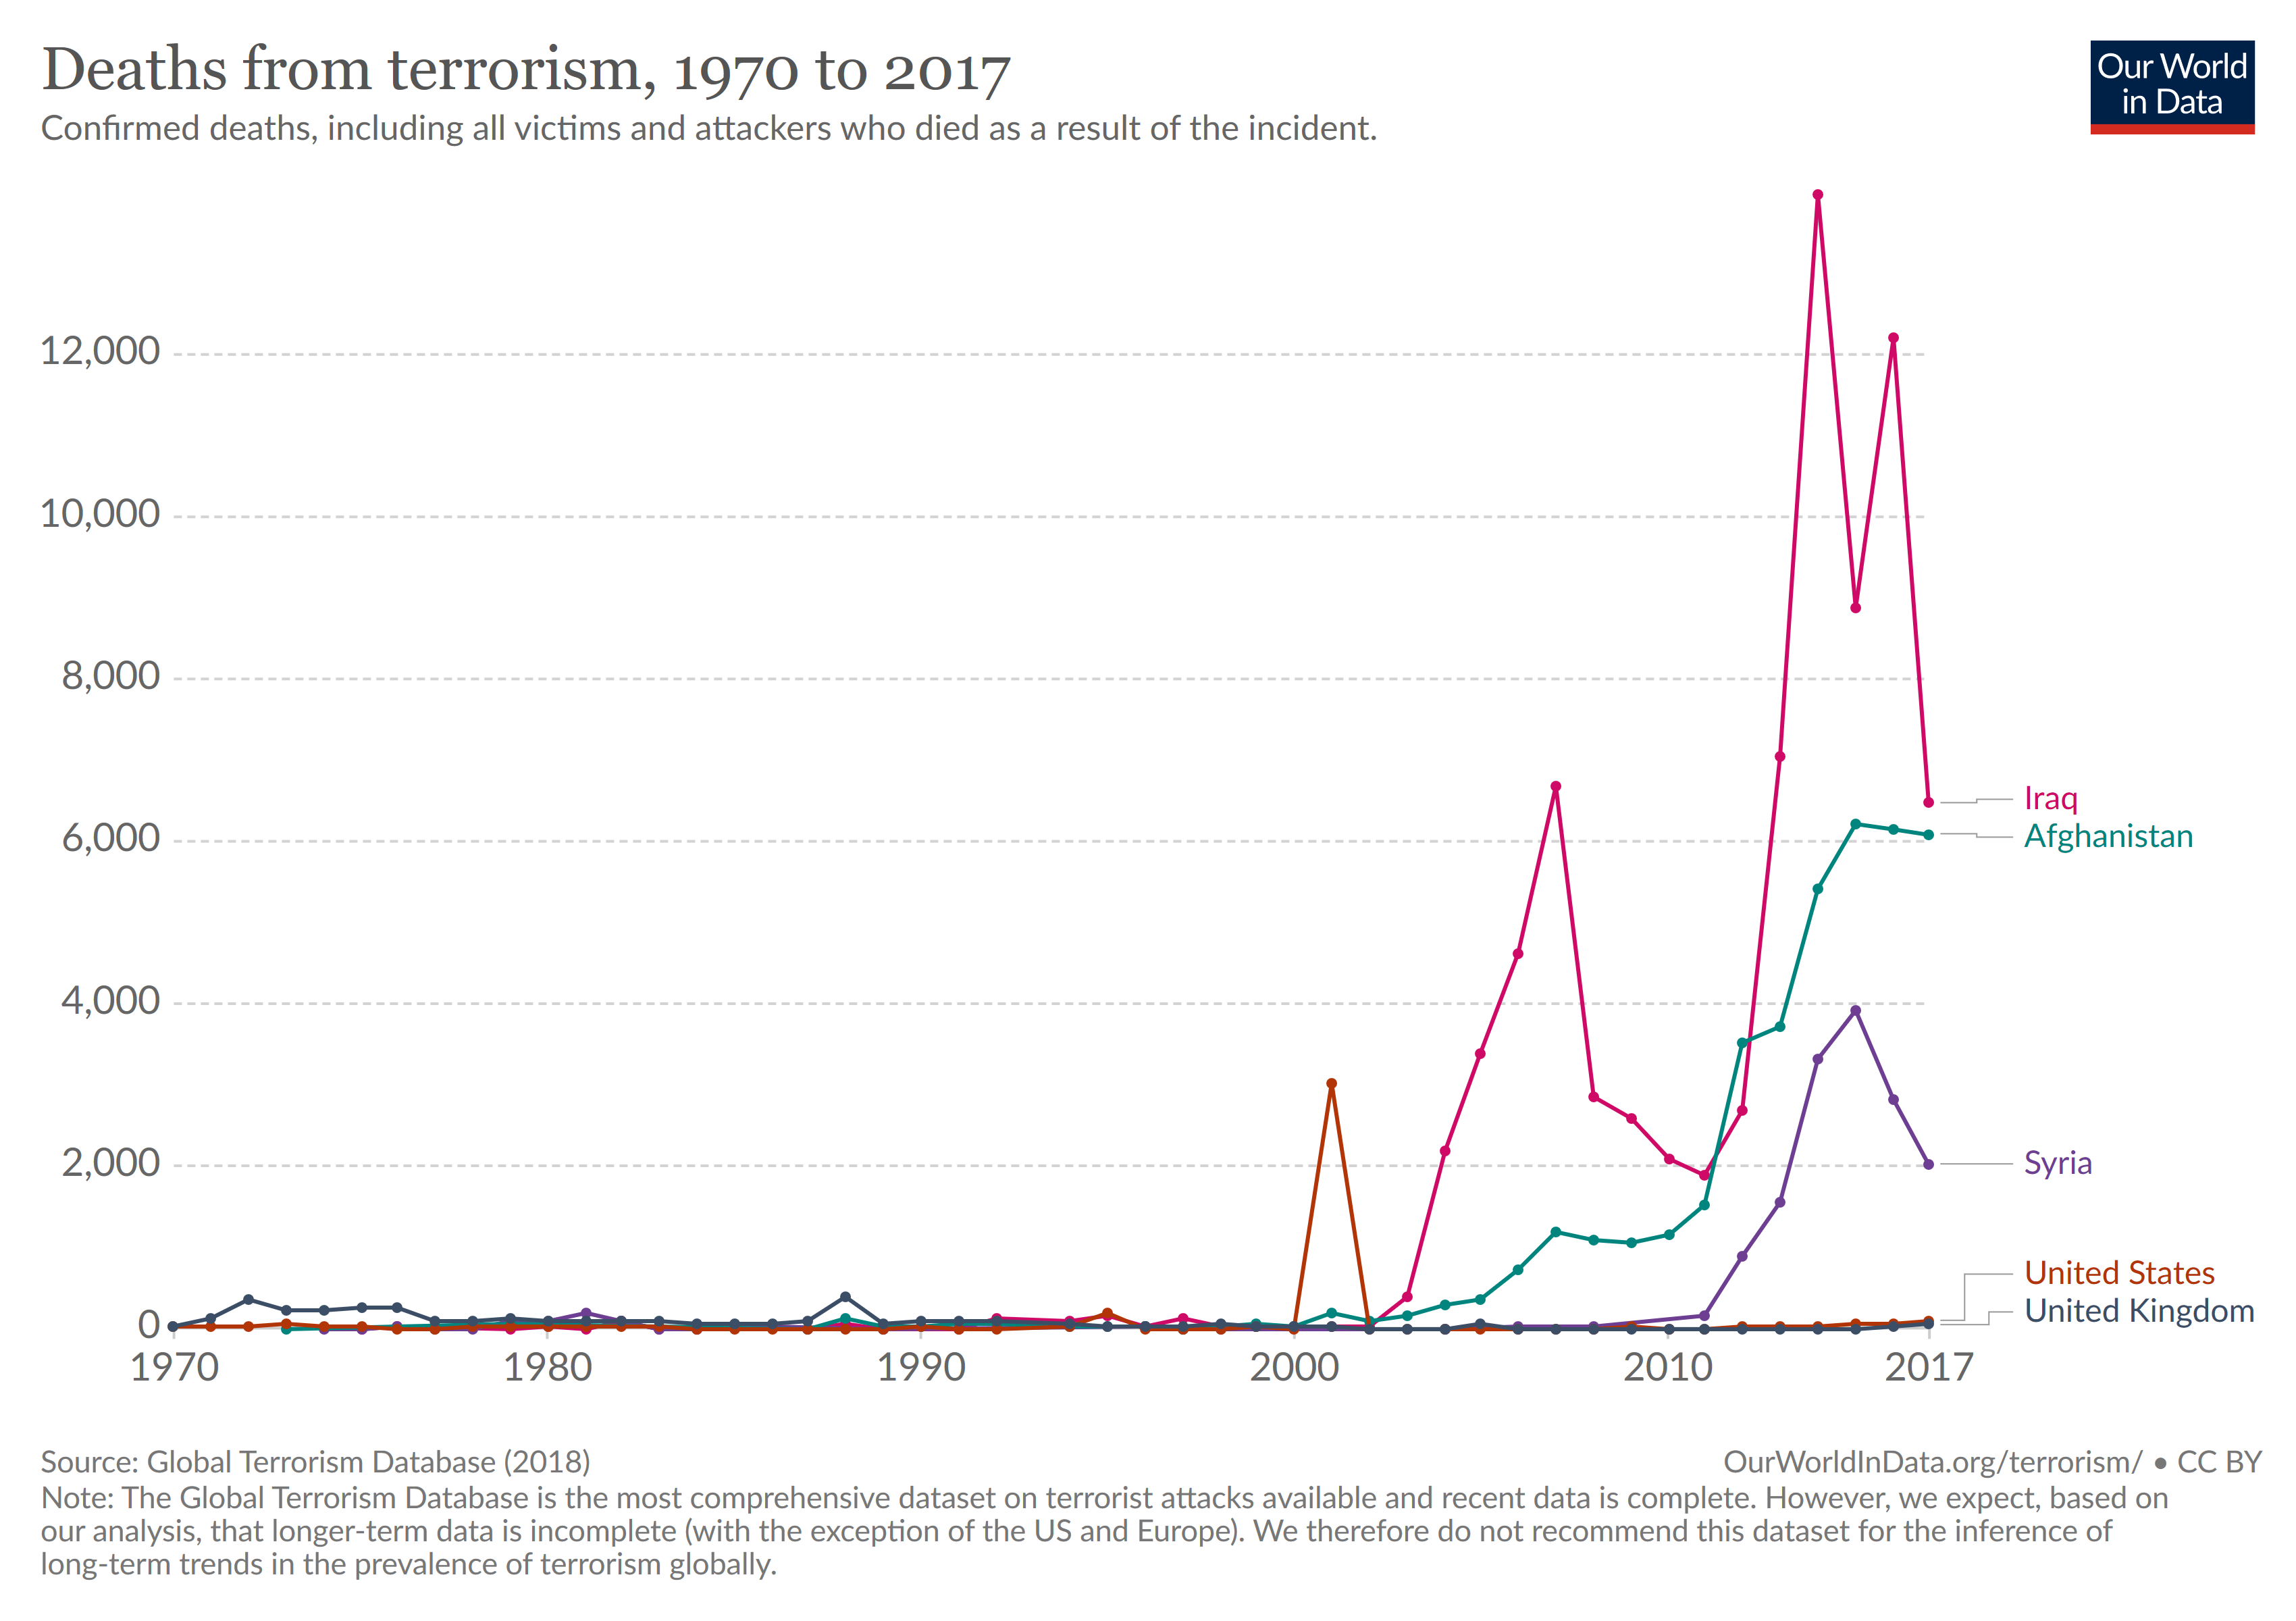
\includegraphics[scale=0.15]{figures/fatalities-from-terrorism}
    \caption{Deaths from terrorism, 1970--2017.}
    \label{fig:appendix_terrorism_deaths}
\end{figure*}\label{subsec:data-verification-after-some-pre-processing-methods}

\end{document}
